\documentclass[a4paper,12pt]{report}

\usepackage[dutch]{babel}           % Nederlands
\usepackage[latin1]{inputenc}       % speciale karakters

\usepackage{palatino} % font
\usepackage{graphicx} % figuren
\usepackage{float} %positie van figuren

\usepackage{titlesec}	%chapter formating

\usepackage[hyperfootnotes=false]{hyperref} % PDF bookmarks

\usepackage{fancyhdr}

\lhead{Brent Van Wynsberge}
\rhead{Project Algoritmen en Datastructuren II}

\renewenvironment{quote}                            % kleinere citaten
               {\list{}{\rightmargin\leftmargin}    %
                \item[]\small}                      %
               {\endlist}                           %

\setlength{\parindent}{0pt}         % indenteringen met witlijn
\setlength{\parskip}{1em}           %

\setlength{\hoffset}{-1cm}          % kleinere marges
\addtolength{\textwidth}{2cm}
\setlength{\voffset}{-1cm}
\addtolength{\textheight}{2cm}

\makeatletter                               % een witlijn tussen
\renewcommand{\footnoterule}{               % voetnoten en tekst
  \vspace{1em}                              %
  \kern-3\p@\hrule\@width.4\columnwidth     %
  \kern2.6\p@}                              %
\makeatother                                %
                                            %
                               
\usepackage[stable]{footmisc}               % pakket voor bep. voetnoten. (voetnoten in titels)

\usepackage{graphicx}   %afbeeldingen

\newcommand{\nroman}{\renewcommand{\thepage}{\roman{page}}\setcounter{page}{0}}     % romeinse nummers
\newcommand{\narabic}{\renewcommand{\thepage}{\arabic{page}}\setcounter{page}{1}}   % arabische nummers

\setcounter{tocdepth}{3} %include subsubsections in toc

\usepackage[linesnumbered,ruled,vlined]{algorithm2e} 		% Algoritmen
\usepackage{algpseudocode}									%
\renewcommand*{\listalgorithmcfname}{Lijst van algoritmen}	%
\renewcommand*{\algorithmcfname}{Algoritme}					%
\renewcommand*{\algorithmautorefname}{algoritme}				%
%%% TITEL EN AUTEUR %%%

\renewcommand{\title}{
			Wachtlijnen \\
			\large Project Algoritmen en Datastructuren II}
\renewcommand{\author}{
\textbf{\large Brent Van Wynsberge} \\
\small 3$^e$ bachelor Informatica, Universiteit Gent \\
\small Algoritmen en Datastructuren II \\
\small Stamnummer: 01201853 \\
}


%%% / / / %%%

\renewcommand{\maketitle}{
\thispagestyle{empty}
\begin{minipage}{3.5in}

\includegraphics{ugent.png}
\end{minipage}
\hfill
\begin{minipage}{3in}
\begin{flushright}
\author
\bigskip
\textbf{\today}
\end{flushright}
\end{minipage}
\vspace{5em}
\vspace*{\fill}
\begin{center}
\Huge{\title}
\end{center}
\vspace*{\fill}}

\titleformat{\chapter}{\normalfont\huge}{\thechapter.}{20pt}{\huge} %chapterformat

\newcommand{\bigO}[1]{$\bm{\mathcal{O}(#1)}$} %big O notatie

\usepackage{bm}


\begin{document}
\global\emergencystretch = .3\hsize

%%% INLEIDEND %%%
\nroman
\maketitle
\newpage

\tableofcontents
\newpage

\pagestyle{fancy}

%%% HOOFDSTUKKEN %%%
\newpage
\narabic

\chapter{Algoritmen} %bespreking complexiteit en algoritmen
\section{Algemeen}
Aangezien het belangrijk is om de prioriteiten voor elke wachtlijn aan te kunnen passen is het nodig om elke referentie naar het effectieve element zo effici\"ent mogelijk bij te houden. Daarom is het het beste om de referenties naar de elementen en de effectief achterliggende datastructuur afzonderlijk bij te houden. \\ 
Zo kan de elementwijzer gewoon naar een nieuwe datastructuurwijzer wijzen indien deze aangepast wordt en moeten eventuele andere elementen die naar het gewijzigde element niet aangepast worden. \\ \\ %P
De kost voor deze keuze is natuurlijk extra gebruik van het geheugen, maar we zullen later opmerken dat waar de geheugenkost het grootst is ook de tijdscomplexiteit veel beter wordt. \\ \\ %P
Omdat het effici\"ent opslaan van deze wijzers zo belangrijk is wordt dit bij elk algoritme verder besproken. %P \\ \\
Voor het aanpassen van de elementen maken we telkens het onderscheid tussen twee gevallen: het verhogen van een element en verlagen van een element. Dit omdat ze beide verschillende gevolgen hebben en het verlagen van een element in vele gevallen effici\"enter kan gebeuren dan zijn tegenhanger. %p

\newpage
\section{Binaire hoop}  % BHeap
\subsection{Centrale operaties}
Elke bewerking op de binaire hoop is gebaseerd op 2 operaties: \Call{moveUp}{} en \Call{fixHeap}{}. Daarom geven we hieronder de pseudocode voor deze operaties en tonen we de complexiteit aan.
\subsubsection{moveUp}
\begin{algorithm}[H]
\caption{moveUp}
\SetAlgoLined	
\DontPrintSemicolon
$element \gets elementToMove$\;
\While{$hasParent(element) \land parent > element$}{
\Call{swap}{element, parent}\;
$element \gets parent$\;
}
\end{algorithm}
De \Call{swap}{} operatie wisselt de elementen en hun indexen om in \bigO{1} tijd. \\
In het slechtste geval verplaatst \Call{moveUp}{} een blad naar de wortel. Deze operatie heeft dus een complexiteit \bigO{\log n}.
\subsubsection{fixHeap}
\begin{algorithm}[H]
\caption{fixHeap}
\SetAlgoLined	
\DontPrintSemicolon
$element \gets elementToMove$\;
\While{$hasChild(element)$}{
$min \gets smallest(leftChild(element), rightChild(element))$\;
\If{$element \leq min$}{
\Return\;}
\Call{swap}{element, min}\;
$element \gets min$\;
}
\end{algorithm}
In het slechtste geval wordt hier de wortel naar een blad verplaatst wat ook een complexiteit \bigO{\log n} heeft.
\subsection{Element verlagen}
\begin{algorithm}[H]
\caption{decreaseElement}
\SetAlgoLined	
\DontPrintSemicolon
$element.value \gets newValue$\;
\Call{moveUp}{element.index}\;	
\end{algorithm}
We zien direct dat \Call{moveUp}{} hier de duurste operatie is en we hebben al eerder aangetoond wat zijn complexiteit is. Deze operatie heeft dus complexiteit \bigO{\log n}.
\subsection{Element verhogen}
\begin{algorithm}[H]
\caption{increaseElement}
\SetAlgoLined	
\DontPrintSemicolon
$element.value \gets newValue$\;
\Call{fixHeap}{element.index}\;		
\end{algorithm}
Analoog met hierboven heeft deze operatie een complexiteit \bigO{\log n}.
\subsection{Element verwijderen}
\begin{algorithm}[H]
\caption{deleteElement}
\SetAlgoLined	
\DontPrintSemicolon
$element.value \gets -\infty$\;
\Call{moveUp}{element.index}\;	
\Call{removeMin}{ }\;
\end{algorithm}
Hier geven we het element de kleinst mogelijke waarde zodat het in de wortel terechtkomt als we de \Call{moveUp}{} operatie uitvoeren (in de praktijk geven we met een boolean aan dat we het element in de wortel willen). Nadien verwijderen we de wortel uit de binaire hoop. \\
We weten reeds dat \Call{moveUp}{} complexiteit \bigO{\log n} heeft. \\ \\
In Algoritmen en Datastructuren I hebben we reeds aangetoond dat de \Call{removeMin}{} operatie ook complexiteit \bigO{\log n} heeft. We kunnen dit hier ook eenvoudig inzien omdat bij \Call{removeMin}{} het laatste blad de nieuwe wortel wordt en dan \Call{fixHeap}{} op deze wortel wordt toegepast. \\ \\
Dus ook deze operatie heeft complexiteit \bigO{\log n}.
\subsection{Bijhouden van wijzers}
Het bijhouden van de locatie van het element binnen de datastructuur is erg goedkoop. Aangezien de binaire hoop in arrayvorm opgeslagen wordt volstaat het om bij elk element een index bij te houden. \\ \\
Wanneer we dit element willen aanpassen weten we direct waar in het array het element zich bevindt en besparen we de kost van het opzoeken van het element. Als we dit element verplaatsen kunnen we gewoon de index binnen het element object aanpassen. Dit kan natuurlijk in \bigO{1} tijd. 

\newpage
\section{Binomiale wachtlijn} % Prio queue
Later in deze sectie zullen we het bijhouden van de wijzers uitgebreider bespreken. Voor het beschrijven van het algoritme zullen we dit echter achterwege laten en een element ook als wijzer naar zijn locatie binnen de datastructuur beschouwen. \\
Dit omdat er een 'HashMap' bijgehouden wordt met de element referenties naar de locatiereferenties. We weten echter dat de \Call{get}{} operatie op een 'HashMap' in \bigO{1} tijd gebeurt en kunnen deze operaties dus verwaarlozen.
\subsection{Centrale operaties}
De meest belangrijke operatie op een binomiale wachtlijn is de \Call{merge}{} operatie, deze staat al beschreven in de cursus en er werd reeds aangetoond dat deze in \bigO{\log n} tijd gebeurt.\footnote{pg.~60} \\ \\
We breiden de wachtlijn echter nog verder uit met 2 operaties om het aanpassen van elementen ook mogelijk te maken.
\subsubsection{moveUp}
\begin{algorithm}[H]
\caption{moveUp}
\SetAlgoLined	
\DontPrintSemicolon
$node \gets elementToMove$\;
\If{$\neg hasParent(node)\lor node \geq node.parent$}{\Return\;}
\Call{swap}{node, node.parent}\;
\Call{moveUp}{node}\;
\end{algorithm}
Net zoals bij het vorige algoritme heeft de \Call{swap}{} operatie hier ook \bigO{1} dankzij het gebruik van de 'HashMap' om de referenties op te slaan. \\ \\
We weten van dit algoritme dat het enkel gebruik maakt van de ouder van het element.
Er wordt niet gekeken naar andere bomen in de wachtrij, dus in het slechtste geval verplaatst deze het diepste blad in de grootste boom naar de wortel van die boom. \\ \\
In de cursus is reeds gesteld dat als de wachtlijn $n$ toppen heeft er een boom met diepte $k$ $\Longleftrightarrow$ de $k\textsuperscript{de}$ bit van de binaire voorstelling 1 is.\footnote{\textbf{Lemma 11}, pg.~59} \\
En we hebben in de cursus ook reeds aangetoond dat $\log n$ een bovengrens is voor de grootste diepte van een boom in de wachtlijn.\footnote{\textbf{Het kleinste element vinden}, hoogste diepte, pg.~59} \\ \\
Dit algoritme heeft dus een complexiteit \bigO{\log n}.
\subsubsection{moveDown}
\begin{algorithm}[H]
\caption{moveDown}
\SetAlgoLined	
\DontPrintSemicolon
$node \gets elementToMove$\;
\If{$\neg hasChildren(node)$}{\Return\;}
$min \gets \Call{min}{node.children}$\;
\If{$min \geq node$}{\Return\;}
\Call{swap}{node, min}\;
\Call{moveDown}{node}\;
\end{algorithm}
We bespreken eerst de complexiteit van de \Call{min}{} operatie. In het slechtste geval wordt de \Call{min}{} operatie opgeroepen op de wortel van de hoogste boom in de wachtlijn. \\
We weten dat die wortel net zoveel kinderen heeft als zijn hoogte, gezien de binomiaaleigenschap. \\ In het slechtste geval moet de \Call{min}{} operatie dus $\log n$ elementen overlopen. \Call{min}{} heeft dus een complexiteit van \bigO{\log n}. \\ \\
Gelijkaardig met eerder zal de \Call{moveDown}{} operatie $\log n$ keer overlopen worden als we vertrekken in de wortel en blijven wisselen in de diepste deelboom. \\ \\
We kunnen dus besluiten dat het \Call{moveDown}{} algoritme een complexiteit \bigO{{\log}^2 n} heeft. \\
Dit is een stuk minder effici\"ent dan het \Call{moveUp}{} algoritme.

\subsection{Element verlagen}
\begin{algorithm}[H]
\caption{decreaseElement}
\SetAlgoLined	
\DontPrintSemicolon
$element.value \gets newValue$\;
\Call{moveUp}{element}
\end{algorithm}
Deze operatie heeft dus een complexiteit \bigO{\log n}.

\subsection{Element verhogen}
\begin{algorithm}[H]
\caption{increaseElement}
\SetAlgoLined	
\DontPrintSemicolon
$element.value \gets newValue$\;
\Call{moveDown}{element}\;
\end{algorithm}
Deze operatie heeft een complexiteit \bigO{{\log}^2 n}. \\
We kunnen deze operatie echter verder optimaliseren door het element eerst uit de heap te halen en het dan opnieuw te mergen. We beschrijven het algoritme hieronder.
\subsubsection{Alternatief}
\begin{algorithm}[H]
\caption{decreaseElementAlternative}
\SetAlgoLined	
\DontPrintSemicolon
\Call{removeElement}{ }\;
$element.value \gets newValue$\;
\Call{insert}{element}\;
\end{algorithm}
Hieronder staat bewezen dat \Call{removeElement}{} complexiteit \bigO{\log n} heeft. In de cursus\footnote{\textbf{Bewerking: een sleutel toevoegen},~pg.~60} werd al bewezen dat de \Call{insert}{} bewerking complexiteit \bigO{\log n} heeft. \\
De complexiteit van deze alternatieve operatie is dus \bigO{\log n}. Dit is de versie die ge\"implementeerd is.

\subsection{Element verwijderen}
\begin{algorithm}[H]
\caption{removeElement}
\SetAlgoLined	
\DontPrintSemicolon
$element.value \gets -\infty$\;
\Call{moveUp}{element}\;
\Call{removeMin}{ }\;
\end{algorithm}
Deze operatie bestaat dus uit een \Call{moveUp}{} om het element in de wortel te krijgen, gevolgd door een \Call{removeMin}{} om het uit de wachtlijn te krijgen. \\
In de cursus is reeds bewezen dat de \Call{removeMin}{} operatie complexiteit \bigO{\log n} heeft.\footnote{\textbf{Het kleinste element verwijderen}, pg.~62-63} \\
Hierboven hebben we ook de \bigO{\log n} complexiteit van \Call{moveUp}{} aangetoond. \\ \\
We kunnen dus besluiten dat de \Call{removeElement}{} operatie een complexiteit \bigO{\log n} heeft.
\subsection{Bijhouden van wijzers}
De wachtlijn houden we bij in een gelinkte lijst van toppen. Voor elke top houden we telkens het eerste kind bij (als dit er is) en houden we in het kind een gelinkte lijst van de buren van dat kind bij. \\
Indien de top een ouder heeft houden we deze ook bij zodat we eenvoudig de heap kunnen navigeren. \\
Wat direct opvalt is dat er per top vrij veel referenties zijn en dat deze omwisselen snel een complexe (en dure) aangelegenheid kan worden. \\ \\
Daarom gebruiken we voor het opslaan van de elementen een tussenobject waar de waarde van het element in opgeslagen wordt. \\ 
Dit object houden we dan ook bij in elke top. Zo kan het vergelijken van twee toppen erg effici\"ent gebeuren (\bigO{1}). \\
Om voor een element snel zijn locatie te vinden hebben we echter nog geen effici\"ente oplossing. Daarom slaan we voor elk element een referentie naar de bijhorende top op in een 'HashMap'. \\ \\
Op die manier kunnen we de locatie van een element in \bigO{1}\footnote{Ervan uitgaande dat de hashfunctie voldoende goed presteert.} tijd vinden. \\
Indien een element verplaatst wordt is het ook erg snel om deze aanpassing door te voeren. We plaatsen gewoon de nieuwe top op de plaats van het element in de 'HashMap' wat ook in \bigO{1} tijd verloopt.



\newpage
\section{Leftist heap}
Ook hier leek het afzonderen van de elementen met hun locatie in de leftis heap aanvankelijk beter dan de referenties telkens om te wisselen. Deze keer is het echter wel mogelijk om in \bigO{1} tijd referenties om te wisselen dus moet er nog verder ge\"experimenteerd worden om te zien of dit geen sneller resultaat zou opleveren.
\subsection{Centrale operaties}
Ook bij de Leftist heap is de \Call{merge}{} operatie de bewerking die aan de basis ligt van de meeste interacties met de wachtlijn. In de cursus hebben we bewezen dat deze complexiteit \bigO{\log n} heeft.\footnote{\textbf{lemma 15}, pg.~68} \\
Verder introduceren we wederom 2 basisoperaties om een element binnen de hoop te verplaatsen.
\subsubsection{moveUp}
\begin{algorithm}[H]
\caption{moveUp}
\SetAlgoLined	
\DontPrintSemicolon
$node \gets elementToMove$\;
\While{$hasParent(node)\land node.parent>node$}{
\Call{swap}{node, node.parent}\;
}
\end{algorithm}
We kunnen hier weer opmerken dat het slechtste geval zich voordoet wanneer het diepste blad naar de wortel verplaatst moet worden.
Echter is de Leftist boom geen gewone binaire boom en kan het zijn dat door de leftist eigenschap de boom bestaat uit \'e\'en lang pad van enkel linkerkinderen langs de wortel. \\ \\
De \Call{moveUp}{} operatie voor een leftist heap heeft dus een complexiteit \bigO{n}. \\ 
Dit is de duurste \Call{moveUp}{} die we tot nu toe gezien hebben.

\subsubsection{moveDown}
\begin{algorithm}[H]
\caption{moveDown}
\SetAlgoLined	
\DontPrintSemicolon
$node \gets elementToMove$\;
$min \gets \Call{min}{node.left, node.right}$\;
\If{$min >= node$}{\Return\;}
\Call{swap}{min, node}\;
\Call{moveDown}{node}\;
\end{algorithm}
Analoog met hierboven heeft deze operatie ook complexiteit \bigO{n}. \\

\subsection{Element verlagen}
\begin{algorithm}[H]
\caption{decreaseElement}
\SetAlgoLined	
\DontPrintSemicolon
$element.value \gets newValue$\;
\Call{moveUp}{element}
\end{algorithm}
Deze operatie heeft dus complexiteit \bigO{n}.

\subsection{Element verhogen}
\begin{algorithm}[H]
\caption{increaseElement}
\SetAlgoLined	
\DontPrintSemicolon
$element.value \gets newValue$\;
\Call{moveDown}{element}\;
\end{algorithm}
Ook deze operatie heeft complexiteit \bigO{n}.

\subsection{Element verwijderen}
\begin{algorithm}[H]
\caption{removeElement}
\SetAlgoLined	
\DontPrintSemicolon
$element.value \gets -\infty$\;
\Call{moveUp}{element}\;
\Call{removeMin}{ }\;
\end{algorithm}
De \Call{moveUp}{} operatie heeft complexiteit \bigO{n}, zoals eerder aangetoond. \\
De \Call{removeMin}{} operatie heeft complexiteit \bigO{\log n} aangezien dit gewoon het mergen van 2 leftist heaps inhoudt. \\ \\ 
De \Call{removeElement}{} operatie heeft dus complexiteit \bigO{n}.

\subsection{Bijhouden van wijzers}
Net als bij de binomiale wachtlijn slaan we hier ook weer een referentie naar het Element afzonderlijk op binnen de top, en vice versa via de 'HashMap'. \\ 
Zoals eerder vermeld kan het omwisselen van de referenties van toppen echter in \bigO{1} gebeuren en moet er dus verder getest worden of dit implementeren aanzienlijk sneller zou verlopen dan de 'HashMap' gebruiken.
%%%%Skew
\newpage
\section{Skew heap}
De skew heap lijkt erg op de leftist heap. Het voldoet aan praktisch dezelfde voorwaarden als een leftist heap, maar probeert gebalanceerd te blijven door bij elke merge bewerking de kinderen om te wisselen en niet alleen wanneer er niet meer aan de voorwaarde voldaan wordt. \\
De gebruikte algoritmes zullen dan ook redelijk analoog lopen met de leftist heap.
\subsection{Centrale operaties}
De centrale operatie bij deze heap is ook weer de \Call{merge}{} operatie. Deze heeft een geamortiseerde complexiteit van \bigO{\log n}. \\
Gezien de gelijkenissen met de skew heap gebruiken we ook dezelfde operaties.
\subsection{moveUp}
\begin{algorithm}[H]
\caption{moveUp}
\SetAlgoLined	
\DontPrintSemicolon
$node \gets elementToMove$\;
\While{$hasParent(node)\land node.parent>node$}{
\Call{swap}{node, node.parent}\;
}
\end{algorithm}
Ook voor de boomstructuur van de skew heap is er geen bovengrens voor de diepte. Deze operatie heeft dus complexiteit \bigO{n}.
\subsubsection{moveDown}
\begin{algorithm}[H]
\caption{moveDown}
\SetAlgoLined	
\DontPrintSemicolon
$node \gets elementToMove$\;
$min \gets \Call{min}{node.left, node.right}$\;
\If{$min >= node$}{\Return\;}
\Call{swap}{min, node}\;
\Call{moveDown}{node}\;
\end{algorithm}
Net als hierboven heeft deze operatie complexiteit \bigO{n}.
\subsection{Element verlagen}
\begin{algorithm}[H]
\caption{decreaseElement (\bigO{n})}
\SetAlgoLined	
\DontPrintSemicolon
$element.value \gets newValue$\;
\Call{moveUp}{element}
\end{algorithm}
\subsection{Element verhogen}
\begin{algorithm}[H]
\caption{increaseElement (\bigO{n})}
\SetAlgoLined	
\DontPrintSemicolon
$element.value \gets newValue$\;
\Call{moveDown}{element}
\end{algorithm}
\subsection{Element verwijderen}
\begin{algorithm}[H]
\caption{removeElement}
\SetAlgoLined	
\DontPrintSemicolon
$element.value \gets -\infty$\;
\Call{moveUp}{element}\;
\Call{removeMin}{ }\;
\end{algorithm}
\Call{removeMin}{} heeft complexiteit \bigO{\log n} aangezien dit het mergen van beide kinderen inhoudt. De complexiteit van de \Call{moveUp}{} operatie hebben we reeds aangetoond. \\
Deze operatie heeft complexiteit \bigO{n}.
\subsection{Bijhouden van wijzers}
Het bijhouden van de wijzers verloopt helemaal analoog met de leftist heap, aangezien enkel de merge bewerkingen verschillen en deze geen gebruik maakt van de wijzers naar het element.
%%%%Pairing
\newpage
\section{Pairing heap}
Deze heap is een interessante heap omdat het merged in \bigO{1} tijd. We kunnen dus vaker gebruik maken van de merge operatie omdat deze relatief goedkoop is.
\subsection{Centrale operaties}
De \Call{merge}{} operatie van de pairing heap heeft complexiteit \bigO{1}. We kunnen dit gemakkelijk inzien als we het algoritme bekijken. \\
\begin{algorithm}[H]
\caption{merge}
\SetAlgoLined	
\DontPrintSemicolon
$min, max \gets$ \Call{compare}{heap1, heap2}\;
$max.sibling \gets min.child$\;
$min.child \gets max$\;
\end{algorithm}

\subsection{Element verlagen}
\begin{algorithm}[H]
\caption{decreaseElement}
\SetAlgoLined	
\DontPrintSemicolon
$node.value \gets newValue$\;
$current \gets node.parent.child$\;
\While{$current.sibling \neq node$}{
$current \gets current.sibling$\;
}
$current.sibling \gets node.sibling$\;
$root \gets $\Call{merge}{root,node}\;
\end{algorithm}
We willen het te verplaatsen element opnieuw mergen met de pairing heap. Op die manier komt de gewijzigde top terug op de juiste plaats in de heap terecht. Dit kan, zoals eerder aangetoond, in \bigO{1} tijd. \\ \\
Alvorens we dit kunnen doen moeten we echter de referentie naar het te verplaatsen element verwijderen uit de heap, door de buur van die top te zoeken. We weten dat we bij het verwijderen van het minimum van de pairing heap voor elk kind van de wortel de referentie naar zijn buur verwijderen en elk kind van een pairing heap node ook een pairing heap (met zijn kinderen) is.  \\ \\
Daarom kunnen we de eerder beschreven bewerking beschouwen als een vereenvoudiging van de \Call{removeMin}{} bewerking zonder effectieve verwijdering. Of we kunnen stellen dat de complexiteit van de \Call{removeMin}{} operatie een bovengrens is voor de hier beschreven bewerking. In de opgave voor het project werd reeds meegegeven dat de gearmortiseerde complexiteit van de \Call{removeMin}{} bewerking \bigO{\log n}\footnote{\textbf{sectie 2.1}~pg.~2} is. \\ \\
De complexiteit van \Call{decreaseElement}{} is dus \bigO{\log n}
\subsection{Element verhogen}
\begin{algorithm}[H]
\caption{increaseElement}
\SetAlgoLined	
\DontPrintSemicolon
$node.value \gets newValue$\;
$newNode \gets$\Call{remove}{node}\;
$node \gets$\Call{merge}{node, newNode}\;
$root \gets$\Call{merge}{node,root}\;
\end{algorithm}
In dit geval verwijderen we de node uit de heap, mergen we hem opnieuw met zijn kinderen en tenslotten mergen we deze met de reeds bestaande heap. \\
Aangezien elk kind van de wortel opnieuw een pairing heap is kunnen we stellen dat de \Call{remove}{} operatie overeenkomt met de \Call{Remove-Min}{} operatie op die heap. De complexiteit van de \Call{Remove-Min}{} operatie voor de gehele heap is dus een bovengrens voor de complexiteit van de \Call{remove}{} operatie.\\ \\
De \Call{increaseElement}{} operatie heeft dus complexiteit \bigO{\log n}.
\subsection{Element verwijderen}
\begin{algorithm}[H]
\caption{removeElement}
\SetAlgoLined	
\DontPrintSemicolon
$newNode \gets$\Call{remove}{node}\;
$root \gets$\Call{merge}{newNode,root}\;
\end{algorithm}
Analoog met hierboven heeft de \Call{removeElement}{} operatie complexiteit \bigO{\log n}.
\subsection{Bijhouden van wijzers}
Aangezien we alle bewerkingen op de elementen zelf via de merge bewerking kunnen doen is het niet noodzakelijk om de link tussen het element en de achterliggende datastructuur op te slaan. En kunnen deze dus samenvallen.

%%%%%%%%%%%%%%%%%%%%%%%%Tests
\chapter{Tests} %bespreking van de testmethodes
Voor de tests wordt er gebruik gemaakt van een abstracte 'HeapTest' klasse. Deze genereert een aantal waarden en voert de test op de gevraagde bewerking uit. Na elke bewerking test de klasse of de heap nog correct is. Dit door de \Call{isValid}{} methode van de heap op te roepen (die elke heap die de interface 'ExtendedHeap' volgt implementeert). \\ \\
Het is ook mogelijk door extra testvoorwaarden mee te geven aan de klasse zolang deze de functionele interface 'BiPredicate' implementeert. Deze zet een 'ExtendedHeap' (uitbreiding van de meegegeven Heap) en een 'ComparableElement' (uitbreiding van het meegegeven Element) om in een boolean, die $\bm{true}$ is als er aan de voorwaarde voldaan wordt. \\ \\
Voor de experimenten is er een 'Benchmark' en 'BenchmarkBuilder' klasse voorzien. Via de builder kunnen verschillende parameters (type heap, operatietype, type dataset, grootte,\dots) ingesteld worden voor de benchmark. Nadien kan de benchmark 'gebuild' worden en kan die gestart worden met de \Call{run}{} methode. De benchmark voert dan alle operaties uit en geeft nadien terug hoelang dit geduurt heeft.

%%%%%%%%%%EXPERIMENTEN
\chapter{Experimenten} %bespreking van de experimenten en vergelijking van de algoritmen
\section{Vergelijking van de algoritmen}
We voeren een aantal experimenten uit op de heaps. We voeren elke operatie uit op elke heap en nadien vergelijken we de looptijd voor datasets van bepaalde grootten. We doen dit met 3 verschillende datasets: oplopende waarden, aflopende waarden en willekeurige waarden (die voor elke heap hetzelfde zijn). Wanneer er niet vermeld wordt welke dataset gebruikt werd is dit de random dataset.
\subsection{Insert}
We merken op de onderstaande grafieken op dat de pairing heap en de binaire hoop erg goed presteren bij insert operaties op de heap. \\
Voor de pairing heap komt dit omdat het mergen/inserten in constante tijd verloopt. \\
Bij de binaire hoop is dit niet het geval, het inserten verloopt namelijk in logaritmische tijd. Maar de binaire hoop heeft een erg lage overhead omdat er enkel een array gebruikt wordt. \\
\begin{figure}[H]
	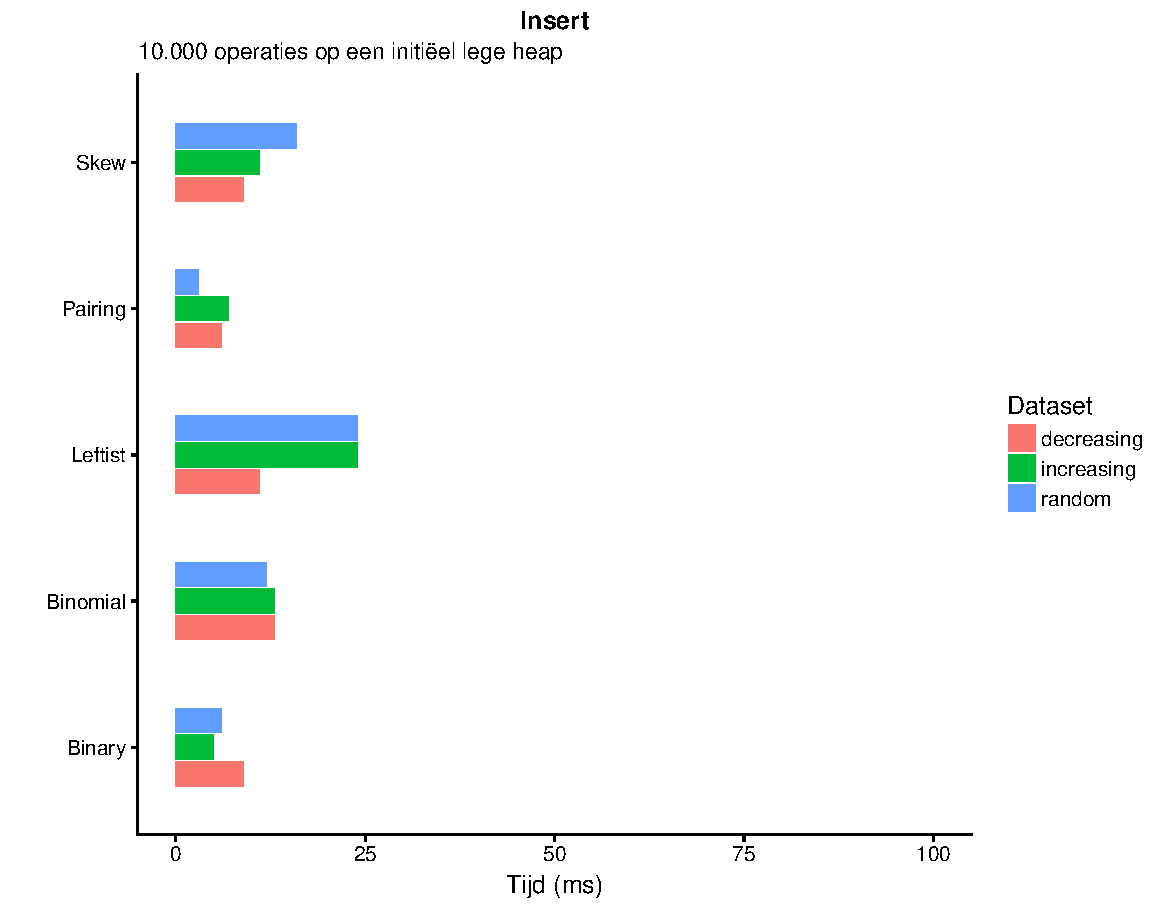
\includegraphics[scale=0.9]{grafieken/insert_10k}
\end{figure}
\begin{figure}[H]
	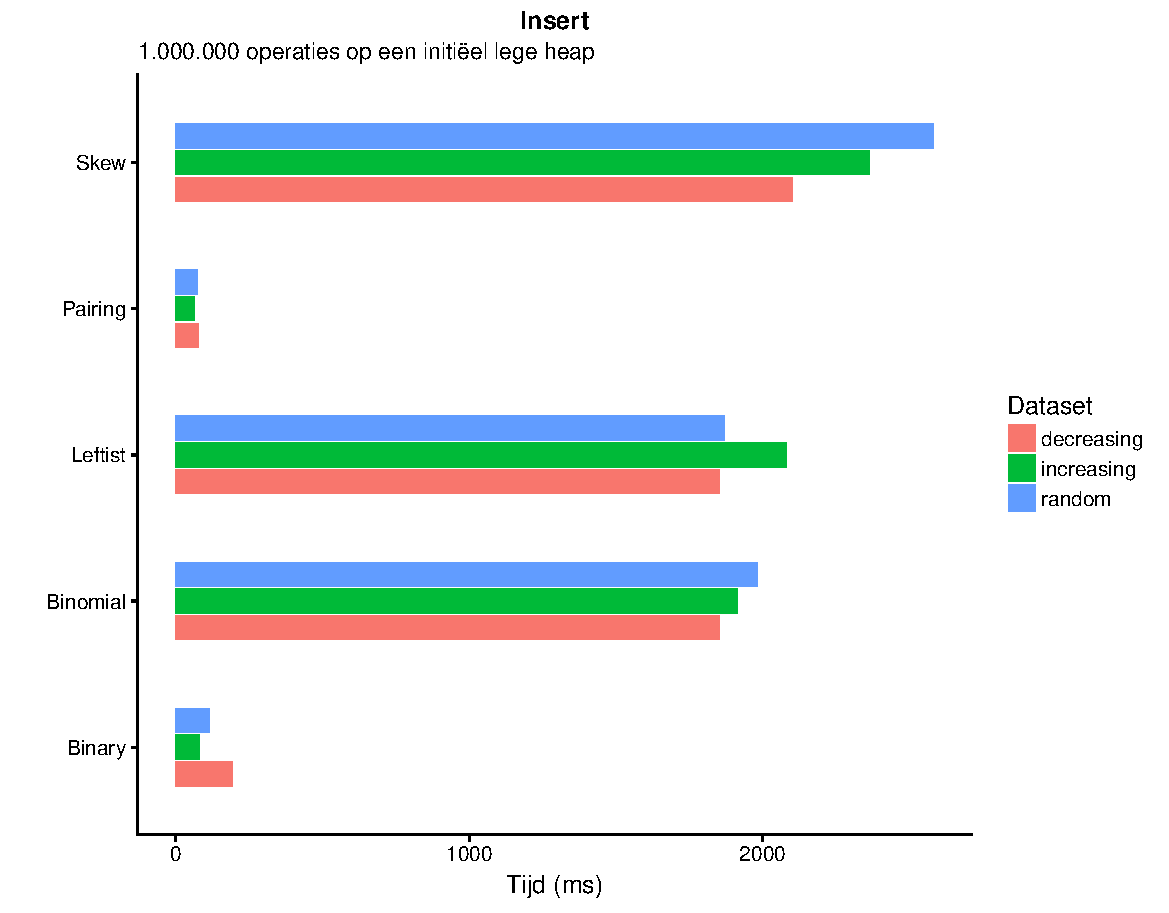
\includegraphics[scale=0.9]{grafieken/insert_1mil}
\end{figure}
\subsection{Remove-Min}
Wanneer we remove-min toepassen zien we dat alle heaps ongeveer dezelfde prestaties hebben. Enkel de pairing heap scoort opvallend slechter dan de rest voor elke dataset. Dit omdat hoewel de complexiteit van elke remove-min operatie logaritmisch is, de operatie voor de pairing heap meer rekenwerk vraagt dan de andere heaps door de opeenvolging van lussen die elk in logaritmische tijd uitvoeren.
\begin{figure}[H]
	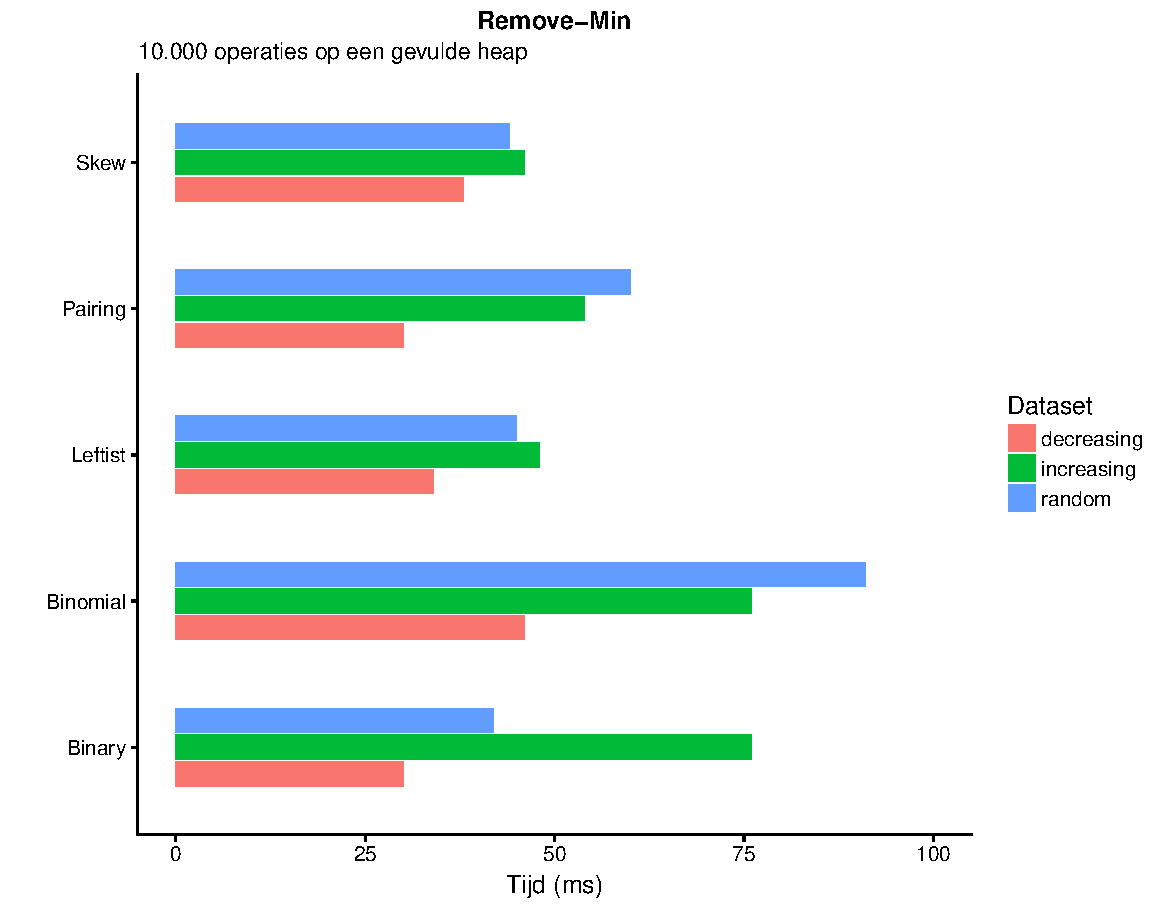
\includegraphics[scale=0.9]{grafieken/remove_min_10k}
\end{figure}
\begin{figure}[H]
	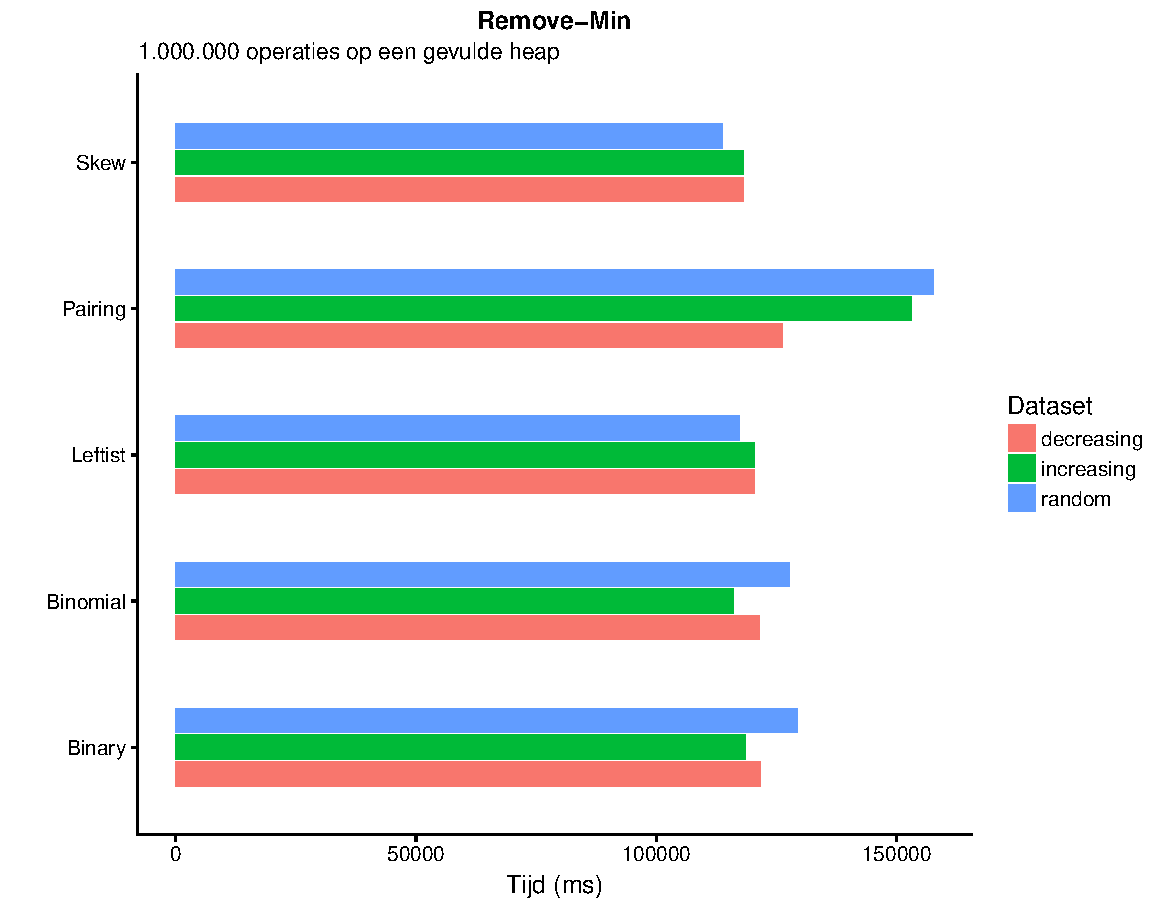
\includegraphics[scale=0.9]{grafieken/remove_min_1mil}
\end{figure}
\subsection{Increase}
Bij de increase operatie vallen er 2 heaps op: \\
De binaire hoop, die weeral dankzij zijn lage overhead erg goede prestaties heeft. \\
En de skew heap omdat deze het slechtste scoort. Het is vooral opvallend dat het verschil tussen de leftist heap en de skew heap zo groot is omdat de increase operaties bijna gelijk verlopen.
\begin{figure}[H]
	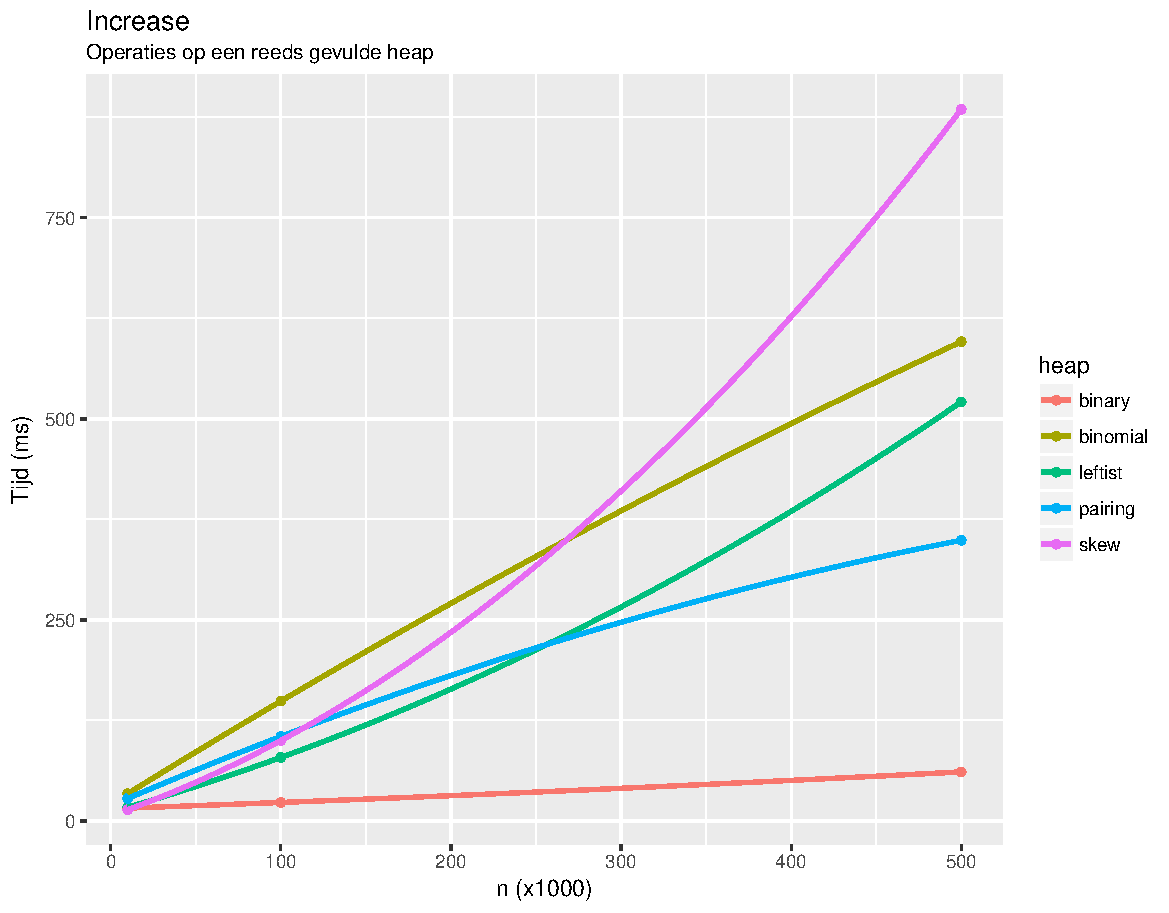
\includegraphics[scale=0.9]{grafieken/increase}
\end{figure}
\subsection{Decrease}
Bij de decrease operatie merken we op dat de skew heap ook weer slecht scoort. Deze heap is een eerste kandidaat voor verder optimalisaties. \\
We zien hier ook dat de pairing heap en de binary heap opvallend goed presteren. Bij de pairing is dit omdat we relatief goedkoop de referentie kunnen verwijderen naar de node en het mergen in constante tijd verloopt. Bij de binaire hoop blijft dezelfde reden gelden.
\begin{figure}[H]
	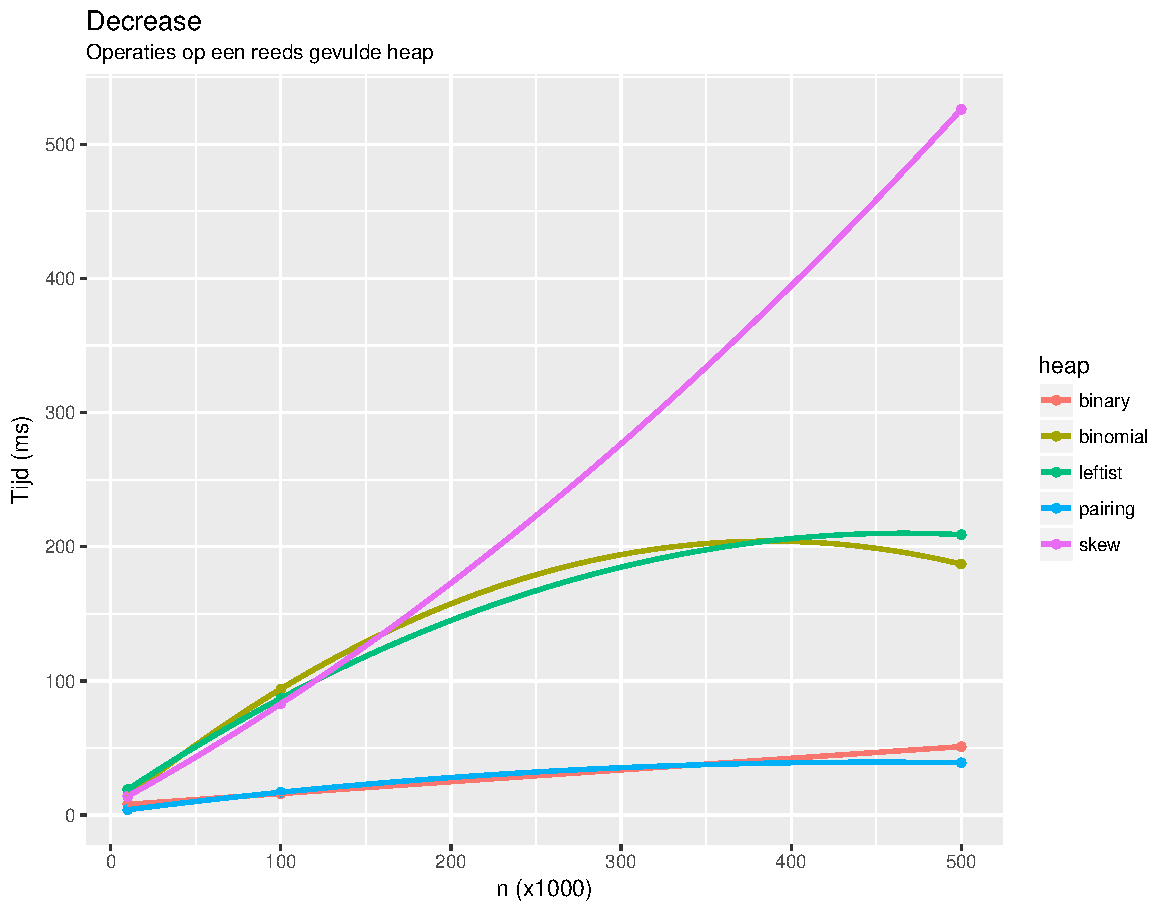
\includegraphics[scale=0.9]{grafieken/decrease}
\end{figure}
\subsection{Remove}
Bij deze operatie merken we op dat de pairing heap enorm slecht scoort. De operatie lijkt zelfs in exponenti\"ele tijd te verlopen. Hoewel dit theoretisch gezien logaritmisch zou moeten zijn.
\begin{figure}[H]
	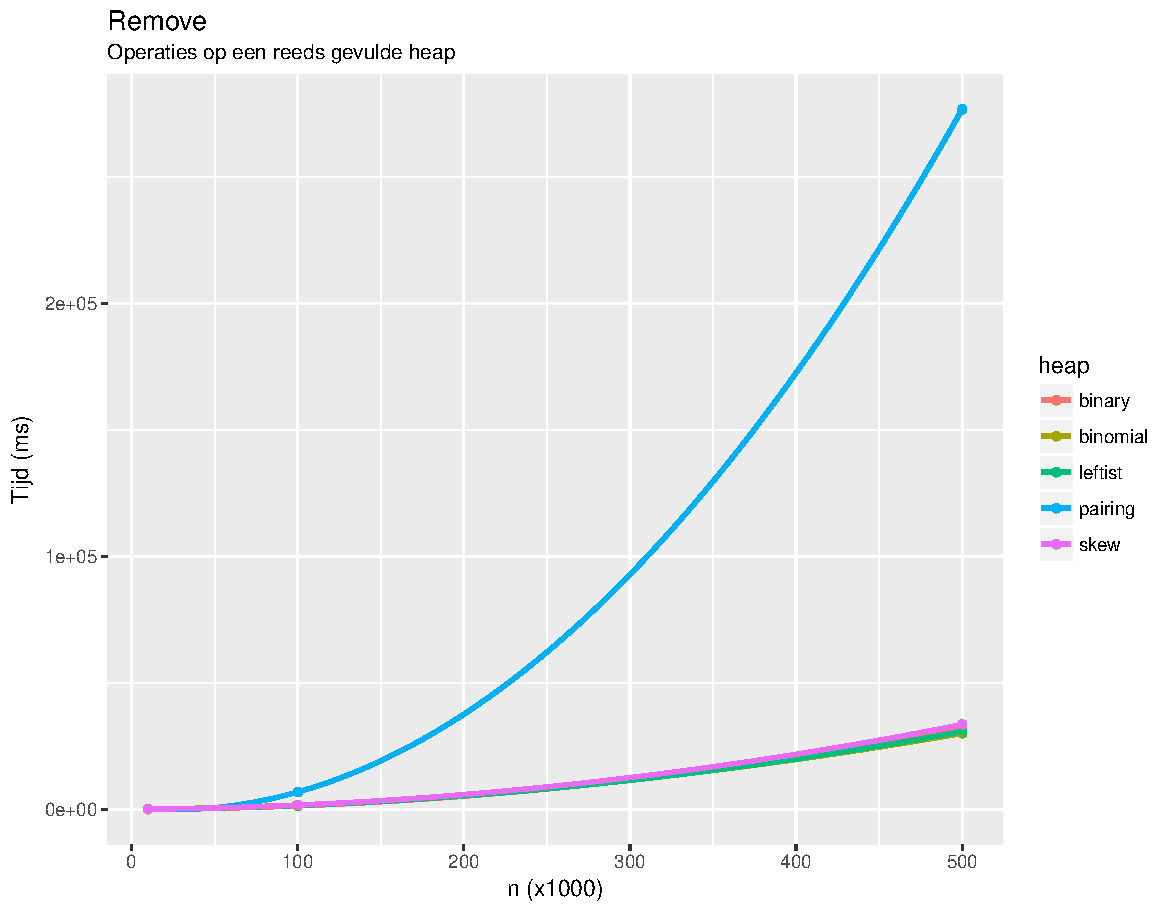
\includegraphics[scale=0.9]{grafieken/remove}
\end{figure}
\subsection{Willekeurig}
In dit experiment voeren we een aantal willekeurige bewerkingen uit op elke heap gevuld met een willekeurige dataset. De bewerkingen zijn dezelfde over elke heap. We merken hier op dat de leftist heap opvallend slechter scoort dan de andere heaps en zelfs de skew heap.
\begin{figure}[H]
	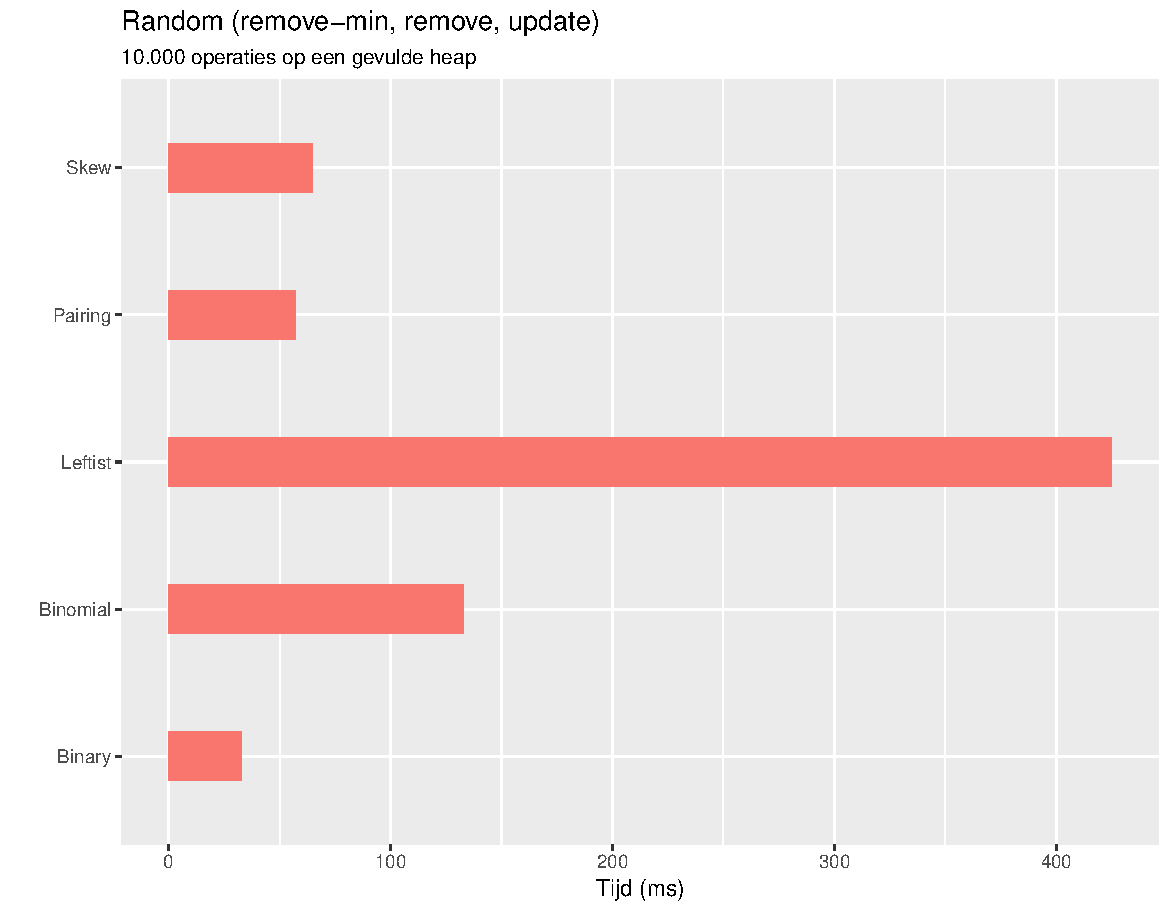
\includegraphics[scale=0.9]{grafieken/random_10k}
\end{figure}
\begin{figure}[H]
	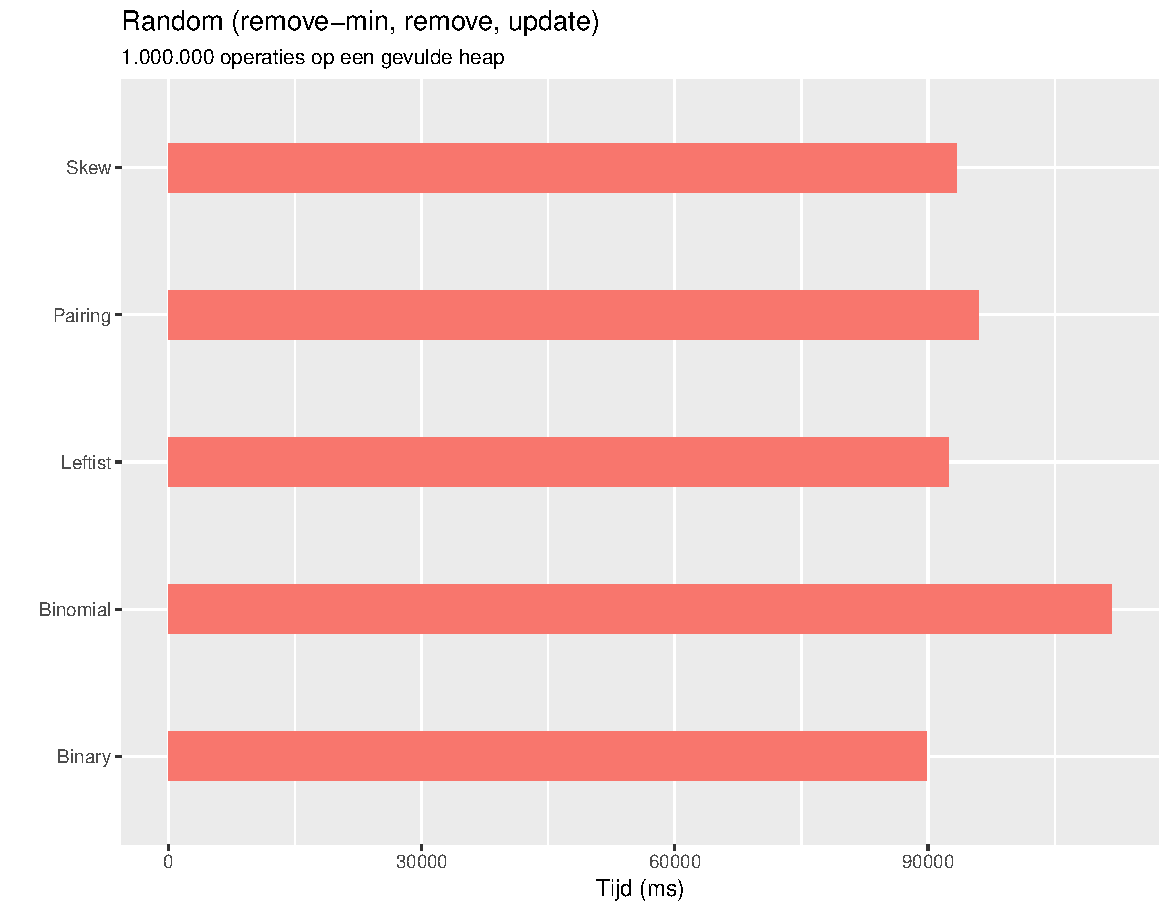
\includegraphics[scale=0.9]{grafieken/random_1mil}
\end{figure}

\chapter{Besluit}
\section{Binaire hoop}
Deze heap is erg goedkoop in effici\"ent. De operaties werken snel, relatief aan de andere heaps. Een nadeel is echter dat het mergen van 2 binaire hopen een erg dure bewerking is.
\section{Binomiale wachtlijn}
Deze heap scoort gemiddeld in elke test. Het voordeel van deze heap is dat wanneer deze voldoende groot is de bewerkingen erg goedkoop kunnen gebeuren (weinig, maar grote bomen in de wachtlijn). Dit heeft wel als gevolg dat sommige bewerkingen, op momenten dat de heap een dure merge bewerking moet doen, veel duurder zijn dan andere.
\section{Leftist- \& Skew heap}
Voor de klassieke heap bewerkingen (insert, remove-min, merge) scoren beide heaps ongeveer hetzelfde. Maar bij de bewerkingen om de prioriteit aan te passen scoort de leftist heap opvallend veel beter dan de skew heap.
\section{Pairing heap}
Deze heap scoort over het algemeen erg goed. Voor de operaties waar er geen verwijderingen plaatsvinden is deze heap superieur aan alle andere heaps (op de binaire hoop na), dit dankzij het mergen in constante tijd. Bij het verwijderen echter liggen de prestaties relatief lager en bij het verwijderen van een arbitrair element lijkt dit zelfs asymptotisch slechter (hoewel dit waarschijnlijk aan een bug moet liggen). Het voordeel dat deze heap heeft tegenover de binaire hoop is dat deze kan mergen in constante tijd. \\
Deze heap zal dan ook in de meeste praktijkgevallen de voorkeur genieten tegenover andere heaps.
\end{document}